\documentclass[12pt]{article}
\usepackage[left=0.25cm,top=1cm,right=0.25cm,bottom=1cm]{geometry}
\textwidth = 20cm
\hoffset = -1cm
\usepackage[utf8]{inputenc}
\usepackage[spanish,es-tabla]{babel}
\usepackage[autostyle,spanish=mexican]{csquotes}
\usepackage[tbtags]{amsmath}
\usepackage{nccmath}
\usepackage{amsthm}
\usepackage{amssymb}
\usepackage{graphicx}
\usepackage{standalone}
\usepackage[outdir=./]{epstopdf}
\usepackage{siunitx}
\usepackage{physics}
\usepackage{color}
\usepackage{float}
\usepackage{multicol}
%\usepackage{milista}
\usepackage{enumitem}
\usepackage{anyfontsize}
\usepackage{anysize}
\usepackage{enumitem}
\usepackage{capt-of}
\usepackage{bm}
\usepackage{relsize}
\usepackage{placeins}
\usepackage{empheq}
\usepackage{cancel}
\usepackage{wrapfig}
\spanishdecimal{.}
\renewcommand{\baselinestretch}{1.5} 
\renewcommand\labelenumii{\theenumi.{\arabic{enumii}}}
\newcommand{\ptilde}[1]{\ensuremath{{#1}^{\prime}}}
\newcommand{\stilde}[1]{\ensuremath{{#1}^{\prime \prime}}}
\newcommand{\ttilde}[1]{\ensuremath{{#1}^{\prime \prime \prime}}}
\newcommand{\ntilde}[2]{\ensuremath{{#1}^{(#2)}}}


\title{Funciones de Bessel} \vspace{-3ex}
\author{M. en C. Gustavo Contreras Mayén}
\date{ }
\newcommand{\Cancel}[2][black]{{\color{#1}\cancel{\color{black}#2}}}
\begin{document}
\vspace{-4cm}
\maketitle
\fontsize{14}{14}\selectfont
\tableofcontents
\newpage

%Referencia Sepúlveda - Lecciones de Física Matemática. Cap. 8 Funciones de Bessel
\section{Las funciones de Bessel.}

Las funciones de Bessel tienen aplicaciones en distintas áreas y problemas de la física: mecánica cuántica, electrodinámica y otras disciplinas.
\par
La ecuación de Bessel surge de la separación de variables de las ecuaciones de Laplace y Helmholtz en coordenadas cilíndricas; la ecuación de Laplace en coordenadas cilíndricas da lugar a las siguientes ecuaciones diferenciales:

\begin{align}
\begin{aligned}
\dv[2]{G(\varphi)}{\varphi} &= - \nu^{2} \, G(\varphi) \\[0.5em]
\dv[2]{Z(z)}{z} &= k^{2} \, Z(z) \\[0.5em]
\dfrac{1}{\rho} \dv{}{\rho} &\left( \rho \, \dv{R(\rho)}{\rho} \right) + \left( k^{2} - \dfrac{\nu^{2}}{\rho^{2}} \right) \, R(\rho) = 0
\end{aligned}
\label{eq:ecuacion_08_02} 
\end{align}

La última de ellas es la ecuación de Bessel. Como un primer paso en su solución conviene definir la nueva variable adimensional $ x = k \, \rho$, que conduce a la siguiente ecuación donde, para generalizar, $\nu$ no es necesariamente entero:
\begin{align}
x^{2} \, \stilde{y} (x) +  x \, \ptilde{y} (x) +  (x^{2} - \nu^{2}) \, y(x) = 0
\label{eq:ecuacion_08_03}
\end{align}

Como $x^{2}$ se anula\footnote{No debemos de descuidar el análisis de los puntos singulares regulares en la ecuación diferencial.} en $x = 0$, se propone resolverla mediante el método de Frobenius, es decir, consideramos que tiene una solución que es una serie de potencias: 
\begin{align*}
y(x) = \sum_{n=0}^{\infty} a_{n} \, x^{n + r}
\end{align*}

por lo que al diferenciar la solución hasta en dos ocasiones
\begin{align*}
\ptilde{y} &= \sum_{n=0}^{\infty} a_{n} \, (n + r) \, x^{n + r - 1} \\[0.5em]
\stilde{y} &= \sum_{n=0}^{\infty} a_{n} \, (n + r) \, (n + r - 1) \, x^{n + r - 2}
\end{align*}

Al reemplazar en la ec. (\ref{eq:ecuacion_08_03}) y factorizando los términos, llegamos a:
\begin{align*}
\sum_{n=0}^{\infty} a_{n} \bigg[ (n + r)^{2} - \nu^{2} \bigg] \, x^{n+r} + \sum_{n=0}^{\infty} a_{n} \, x^{n+r+2} = 0
\end{align*}

Si tomamos en cuenta que para una función $f_{n} (x)$ dependiente del índice $n$, es siempre cierto que se cumple:
\begin{align*}
\sum_{n=0}^{\infty} f_{n} (x) = \sum_{n=-2}^{\infty} f_{n+2} (x)
\end{align*}

por lo que podemos escribir:
\begin{align*}
\sum_{n=-2}^{\infty} a_{n+2} \left[ (n + r + 2)^{2} - \nu^{2} \right] \, x^{n+r+2} + \sum_{n=0}^{\infty} a_{n} \, x^{n+r+2} = 0
\end{align*}

La suma de la izquierda contiene dos términos: $\lambda=-2$ y $\lambda=-1$ que no están en la suma de la derecha, para factorizar los términos de la variable $x$ con el mismo exponente, escribimos entonces:
\begin{align*}
a_{0} \, [r^{2} - \nu^{2}] \, x^{-2+r} &+ a_{1} \, [(r+1)^{2} - \nu^{2}] \, x^{-1+r} + \\[0.5em]
&+ \sum_{n=0}^{\infty} \left\{ a_{n+2} [(n + r + 2)^{2} - \nu^{2}] + a_{n} \right\} \, x^{n + r} = 0
\end{align*}

En consecuencia, como las potencias de $x$ son independientes, la única manera en que la expresión se cumpla, es que los coeficientes de las sumas se anulen, recordemos que $a_{0} \neq 0$:
\begin{align*}
a_{0} \, [r^{2} - \nu^{2}] &= 0 \\[0.5em]
a_{1} \, [(r + 1)^{2} - \nu^{2}] &= 0 \\[0.5em]
a_{n+2} \, [(n + r + 2)^{2} - \nu^{2}] + a_{n} &= 0 \hspace{1cm} n = 0, 1, 2, \ldots
\end{align*}

De la primera ecuación, que representa la ecuación de índices tendremos que:
\begin{align}
r = \pm \nu \hspace{1.5cm} \mbox{con } \nu \geq 0
\label{eq:ecuacion_08_04}
\end{align}

al reemplazar las raíces en la segunda ecuación:
\begin{align*}
a_{1} \, [1 \pm 2 \, \nu] = 0
\end{align*}

de donde se sigue $a_{1} = 0$ pues $1 \pm 2 \, \nu$ es diferente de cero para valores arbitrarios de $\nu$. Se anula sólo en el caso muy particular en que $\nu = 1/2$, con el signo inferior.
\par
Reemplazando $r = + \nu$ en la tercera ecuación, obtenemos la relación de recurrencia:
\begin{align*}
a_{n+2} = - \dfrac{a_{n}}{(n + \nu + 2)^{2} - \nu^{2}} = - \dfrac{a_{n}}{(n + 2)(n + 2 \, \nu + 2)}
\end{align*}

\noindent
como $a_{1} = 0$, resultará que todos los coeficientes con índice impar se anulan. Para los coeficiente pares, que se obtienen haciendo $n = 0, 2, 4, \ldots$ tendremos:
\begin{align*}
a_{2} &= \dfrac{-a_{0}}{2 \, (2 \, \nu + 2)} = \dfrac{-a_{0}}{2 \cdot 2 \, (\nu + 1)} \\[0.75em]
a_{4} &= \dfrac{-a_{2}}{4 \, (2 \, \nu + 4)} = \dfrac{(-1)^{2} \, a_{0}}{2 \cdot 2^{4} \, (\nu + 2)(\nu + 1)} \\[0.75em]
a_{6} &= \dfrac{-a_{4}}{6 \, (2 \, \nu + 6)} = \dfrac{(-1)^{3} \, a_{0}}{2 \cdot 3 \cdot 2^{6} \, (\nu + 3)(\nu + 2)(\nu + 1)} \\[0.75em]
&= \dfrac{(-1)^{3} \, a_{0} \, \Gamma (\nu + 1)}{3! \, 2^{6} \, (\nu + 3)(\nu + 2)(\nu + 1) \, \Gamma (\nu + 1)} \\[0.75em]
&= \dfrac{(-1)^{3} \, a_{0} \, \Gamma (\nu + 1)}{3! \, 2^{6} \, \Gamma (\nu + 3 + 1)}
\end{align*}

En donde vemos que se ha ocupado la función $\Gamma(x)$ vista previamente\footnote{Puedes consultar las notas de trabajo sobre la función Gamma $\Gamma(x)$.} De este modo, es directo probar que:
\begin{align}
a_{2n} = \dfrac{(-1)^{n} \, a_{0} \, \Gamma (\nu + 1)}{2^{2n} \, n! \, \Gamma (\nu + n + 1)}
\label{eq:ecuacion_08_05}
\end{align}

Así, reemplazando en la serie de Frobenius:
\begin{align*}
y(x) &= \sum_{n=0}^{\infty} a_{n} \, x^{n+r} = \sum_{p=0}^{\infty} a_{2n} \, x^{\nu+2n} \\[0.5em]
&= a_{0} \, \Gamma (\nu + 1) \, \sum_{p=0}^{\infty} \dfrac{(-1)^{n} \, x^{\nu+2n}}{2^{2n} \, n! \, \Gamma (\nu + n)} \\[0.5em]
&= a_{0} \, \Gamma (\nu + 1) \, 2^{\nu} \, \sum_{n=0}^{\infty} \dfrac{(-1)^{n}}{n! \, \Gamma (\nu + n + 1)} \left( \dfrac{x}{2} \right)^{\nu+2n} \\[0.5em]
&= a_{0} \, \Gamma (\nu + 1) \, 2^{\nu} \, J_{\nu} (x)
\end{align*}

En lo anterior hemos definido la \emph{función de Bessel} de orden $\nu$ real positivo y argumento $x$, que es solución de la ec. (\ref{eq:ecuacion_08_03}):
\begin{align}
\setlength{\fboxsep}{3\fboxsep}\boxed{
J_{v} (x) = \sum_{n=0}^{\infty} \dfrac{(-1)^{n}}{n! \, \Gamma (\nu + n + 1)} \left( \dfrac{x}{2} \right)^{\nu+2n}}
\label{eq:ecuacion_08_06}
\end{align}

De la expansión (\ref{eq:ecuacion_08_05}) se sigue que la serie es convergente. Es fácil concluir en efecto que:
\begin{align*}
\dfrac{a_{2n+2}}{a_{2p}} = \dfrac{-1}{4 \, (n+1)(\nu + n + 1)} \to 0,\hspace{1.5cm} \mbox{si } n \to \infty
\end{align*}

Ahora bien, volvamos a la ec. (\ref{eq:ecuacion_08_04}). La segunda posibilidad es $r = -\nu$. Reemplazando en la ec. (\ref{eq:ecuacion_08_05}) $\nu$ por $-\nu$ se sigue:
\begin{align*}
a_{2n} = \dfrac{(-1)^{n} \, a_{0} \, \Gamma (-\nu + 1)}{2^{2n} \, n! \, \Gamma (-\nu + n + 1)}
\end{align*}

al reemplazar en la serie de Frobenius podemos definir la función de Bessel de orden $-\nu$ en la forma:
\begin{align}
\setlength{\fboxsep}{3\fboxsep}\boxed{
J_{-v} (x) = \sum_{n=0}^{\infty} \dfrac{(-1)^{n}}{n! \, \Gamma (-\nu + n + 1)} \left( \dfrac{x}{2} \right)^{-\nu+2n}}
\label{eq:ecuacion_08_07}
\end{align}

esta serie es convergente para todos los valores de $x$, si $-\nu + 2n \geq 0$.
\par
De la forma de los exponentes en las ecuaciones (\ref{eq:ecuacion_08_06}) y (\ref{eq:ecuacion_08_07}) es fácil ver que, si $\nu$ no es entero, las series $J_{\nu}(x)$ y $J_{-\nu}(x)$ son diferentes y conforman las dos soluciones linealmente independientes de la ecuación de Bessel. La solución general, para $\nu \neq$ entero, será entonces:
\begin{align*}
y_{\nu}(x) = A \, J_{v}(x) + B \, J_{-\nu} (x)
\end{align*}

Veamos ahora qué ocurre si $\nu$ es un entero $p$. Utilizando la propiedad de la función Gamma $\Gamma (\ell + 1) = \ell !$ con $\ell$ entero, la ecuación (\ref{eq:ecuacion_08_07}) se escribe:
\begin{align*}
J_{-p} (x) = \sum_{n=0}^{\infty} \dfrac{(-1)^{n}}{n! \, (-p + n)!} \left( \dfrac{x}{2} \right)^{-p+2n}
\end{align*}

pero $(-p + n)!$ se hace $\infty$ para $n = 0, 1, \ldots, p-1$, de modo que para esos valores de $n$ los términos correspondientes de la serie se anulan, pues (-entero)! $\to \infty$. La parte de la serie que no se anula empieza con $n = p$ y se expresa como:
\begin{align*}
J_{-p} (x) = \sum_{n=p}^{\infty} \dfrac{(-1)^{n}}{n! \, (-p + n)!} \left( \dfrac{x}{2} \right)^{-p+2n}
\end{align*}

y como 
\begin{align*}
\sum_{n=p}^{\infty} f(n) = \sum_{n=0}^{\infty} f(n + p)
\end{align*}

para cualquier función $f(n)$, tendremos entonces
\begin{align*}
J_{-p} (x) &= \sum_{n=0}^{\infty} \dfrac{(-)^{n+p}}{(n + p)! \, n!} \left( \dfrac{x}{2} \right)^{p+2n} \\[0.5em]
J_{-p} (x) &= (-1)^{n} \, J_{p}(x)
\end{align*}

En consecuencia $J_{p}(x)$ y $J_{-p}(x)$ difieren a lo máximo en un signo. Siendo necesario entonces buscar la segunda solución para $\nu \neq$ entero.

\section{La función de Neumann.}

Con el propósito de obtener una segunda solución a la ecuación de Bessel, escribimos la ecuación de la siguiente forma:
\begin{align*}
\stilde{J}_{\nu} + \dfrac{1}{x} \, \ptilde{J}_{\nu}  + \left( 1 - \dfrac{\nu^{2}}{x^{2}} \right) \, J_{\nu} = 0, \hspace{2cm} \ptilde{J}_{\nu} = \dv{J_{\nu}}{x}
\end{align*}

derivando con respecto a $\nu$, obtenemos:
\begin{align}
\pdv{\stilde{J}_{\nu}}{\nu} + \dfrac{1}{x} \, \pdv{\ptilde{J}_{\nu}}{\nu} + \left( 1 - \dfrac{\nu^{2}}{x^{2}} \right) \, \pdv{J_{\nu}}{\nu} - \dfrac{2 \, \nu}{x^{2}} \, J_{\nu} = 0
\label{eq:ecuacion_08_08} 
\end{align}

y también, cambiando $\nu$ por $-\nu$:
\begin{align}
\pdv{\stilde{J}_{-\nu}}{\nu} + \dfrac{1}{x} \, \pdv{\ptilde{J}_{-\nu}}{\nu} + \left( 1 - \dfrac{\nu^{2}}{x^{2}} \right) \, \pdv{J_{-\nu}}{\nu} - \dfrac{2 \, \nu}{x^{2}} \, J_{-\nu} = 0
\label{eq:ecuacion_08_09} 
\end{align}

De la ec. (\ref{eq:ecuacion_08_08}) multiplicando $-(-1)^{\nu}$ a la ec. (\ref{eq:ecuacion_08_09}):
\begin{align*}
&\dv[2]{x} \left( \pdv{J_{\nu}}{\nu} - (-1)^{\nu} \, \pdv{J_{-\nu}}{\nu} \right) + \dfrac{1}{x} \dv{x} \left( \pdv{J_{\nu}}{\nu} - (-1)^{\nu} \,\pdv{J_{-\nu}}{\nu} \right) + \\[0.5em]
&+ \left( 1 - \dfrac{\nu^{2}}{x^{2}} \right) \left( \pdv{J_{\nu}}{\nu} - (-1)^{\nu}  \, \pdv{J_{\nu}}{\nu} \right) - \dfrac{2 \, \nu}{x^{2}} \, (J_{\nu} - (-1)^{\nu} \, J_{-\nu}) = 0
\end{align*}

Si $\nu = n$, y como $J_{-n} = (-)^{n} \, J_{n}$, el último término se anula; precisamente para ello hicimos este tipo de resta entre (\ref{eq:ecuacion_08_08}) y (\ref{eq:ecuacion_08_09}). Así pues, la función de Neumann $N_{n}(x)$, definida por:
\begin{align}
N_{n} (x) = \dfrac{1}{\pi} \left[ \pdv{J_{\nu}}{\nu} - (-1)^{\nu} \, \pdv{J_{-\nu}}{\nu} \right] \eval_{\nu=n}
\label{eq:ecuacion_08_10}
\end{align}
satisface la ecuación de Bessel:
\begin{align*}
\dv[2]{N_{n}}{x} + \dfrac{1}{x} \, \dv{N_{n}}{x} + \left( 1 - \dfrac{\nu^{2}}{x^{2}} \right) \, N_{n} = 0
\end{align*}

La función $N_{n}(x)$, definida por la ec. (\ref{eq:ecuacion_08_10}), es la segunda solución a la ecuación de Bessel para $\nu =$ entero.
\par
La definición (\ref{eq:ecuacion_08_10}) es válida exclusivamente para $\nu = n =$ entero. Nos proponemos ahora extender esta definición para escribir $N_{\nu} (x)$ con $\nu > 0$.
\par
Observemos ante todo que la ec. (\ref{eq:ecuacion_08_10}) puede escribirse en la forma:
\begin{align*}
N_{n} (x) =  \left\{ \dfrac{\displaystyle \dv{{\nu}} \bigg[ \cos \nu \, \pi \, J_{\nu} (x) - J_{-\nu} (x) \bigg]}{\displaystyle \dv{\nu} \sin \nu \, \pi} \right\}  \bigg\vert_{n=\nu}
\end{align*}

donde $\sin n \, \pi = 0$, $\cos n \, \pi = (-1)^{n}$. Al aplicar la regla de L'Hôpital y al evaluar en $\nu = n$, el cociente anterior es la función:
\begin{align}
N_{n} (x) = \dfrac{\cos \nu \, \pi \, J_{\nu} (x) - J_{-\nu} (x)}{\sin \nu \, \pi}
\label{eq:ecuacion_08_11}
\end{align}

Obsérvese que el límite de $N_{\nu} (x)$ cuando $\nu \to n$ es $0/0$, una indeterminación.
\par
La ecuación (\ref{eq:ecuacion_08_11}) es la definición de la función de Neumann para $\nu$ real. Si $\nu \neq$ entero, $J_{\nu} (x)$ y $J_{-\nu} (x)$ son linealmente independientes, de modo que $N_{\nu}(x)$ es solución linealmente dependiente, y si $\nu =$ entero entonces $N_{n}(x)$ dada por la ec. (\ref{eq:ecuacion_08_10}) es la segunda solución. Una forma en series de (\ref{eq:ecuacion_08_10}) es:
\begin{align*}
N_{n}(x) &= \dfrac{2}{\pi} \left[ \ln \left(\dfrac{x}{2} \right) + \gamma - \dfrac{1}{2} \sum_{p=1}^{n} \dfrac{1}{p} \right] \, J_{n} (x) + \\[0.5em]
&- \dfrac{1}{\pi} \sum_{r=0}^{\infty} (-1)^{r} \, \dfrac{1}{r! \, (n + r)!} \, \left( \dfrac{x}{2} \right)^{n+2r} \, \sum_{p=1}^{r} \left( \dfrac{1}{p} + \dfrac{1}{p + n} \right) + \\[0.5em]
&- \dfrac{1}{\pi} \sum_{r=0}^{n-1} \dfrac{(n - r - 1)!}{r!} \, \left( \dfrac{x}{2} \right)^{-n+2r}
\end{align*}
donde $\gamma$ es la constante de Euler-Mascheroni, definida por:
\begin{align*}
\gamma = \lim_{n \to \infty} \left( \sum_{m=1}^{n} \dfrac{1}{m} - \ln n \right) = 0.57721566
\end{align*}
La solución general de la ecuación de Bessel, es entonces:
\begin{align*}
y_{\nu} (x) = A \, J_{\nu} (x) + B \, N_{\nu} (x) \hspace{1.5cm} \mbox{para $\nu$ real}
\end{align*}

\section{Propiedades de las funciones de Bessel.}
\subsection{Raíces.}

Llámense raíces de las funciones de Bessel a los valores de $x$, designados por $\chi_{\nu n}$ para los cuales $J_{\nu} (\chi_{\nu n}) = 0$. 
\par
Cada función de Bessel de orden $\nu$ presenta un número infinito de ceros, que numeramos con $n = 1, 2, 3, \ldots$. Por tanto los ceros deberán clasificarse con dos índices: El primero señala el orden de la función y el segundo el $n-$ ésimo cero. El valor $\chi = 0$ lo consideramos como una raíz trivial.
\begin{figure}[H]
    \centering
    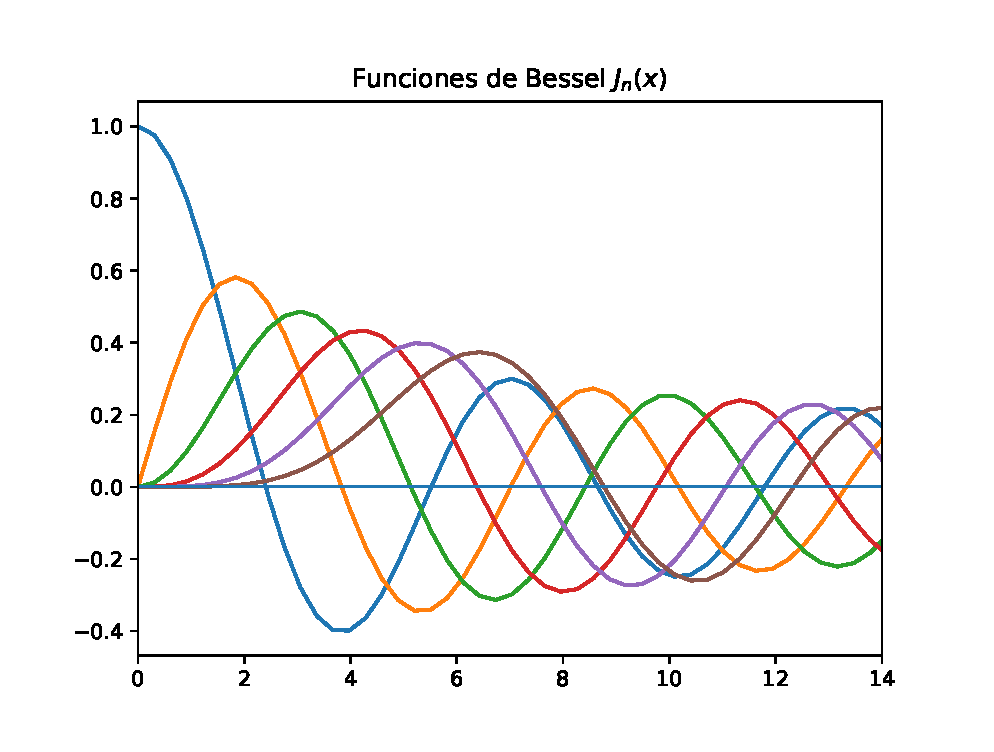
\includegraphics[scale=0.8]{Imagenes/plot_Bessel.eps}
    \caption{Funciones de Bessel de orden $n$, el cruce de cada curva con el eje $y=0$, corresponde a una raíz de la función.}
    \label{fig:figura_Bessel}
\end{figure}

\begin{figure}[H]
    \centering
    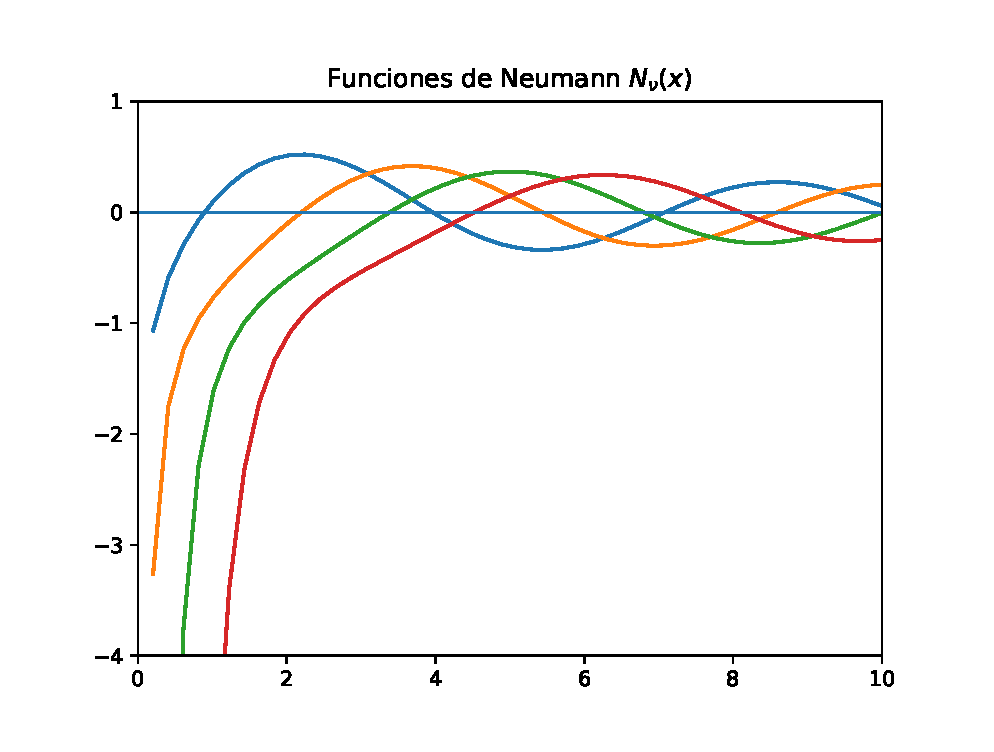
\includegraphics[scale=0.8]{Imagenes/plot_Neumann.eps}
    \caption{Funciones de Neumann de orden $\nu$.}
    \label{fig:figura_Neumann}
\end{figure}

Para $n > -1$ la ecuación $J_{\nu} (x) = 0$ no tiene raíces complejas, ni puramente imaginarias. Además, si $\nu$ es un número real, la ecuación $J_{\nu} (x) = 0$ no tiene raíces comunes ni con $J_{\nu+1} (x) = 0$ ni con $J_{\nu-1} (x) = 0$ (excepto cero). También las funciones de Neumann presentan ceros, como se puede ver en las figuras (\ref{fig:figura_Bessel}) y (\ref{fig:figura_Neumann}), para las funciones de Bessel y Neumann, respectivamente.

\subsection{Relaciones de recurrencia.}

Son expresiones que relacionan entre sí funciones y derivadas de funciones de Bessel de diferente orden.
\par
Por ejemplo, por aplicación directa de la ecuación (\ref{eq:ecuacion_08_06}), se tiene que:
\begin{align*}
J_{\nu-1} (x) - J_{\nu+1} (x)&= 2 \, \dv{J_{\nu}(x)}{x} \\[0.5em]
J_{\nu-1} (x) &= \dfrac{\nu}{x} \, J_{\nu} + \dv{J_{\nu}(x)}{x} \\[0.5em]
J_{\nu-1} &= \left( \dfrac{\nu}{x} + \dv{}{x} \right) \, J_{\nu} \\[0.5em]
J_{\nu+1} &= \left( \dfrac{\nu}{x} - \dv{}{x} \right) \, J_{\nu}
\end{align*}

Estas cuatro ecuaciones son válidas también para $N_{\nu} (x)$. Las dos últimas ecuaciones se deducen de las dos primeras, y aseguran que las funciones de Bessel $J_{\nu \pm 1} (x)$ pueden obtenerse de $J_{\nu}$, mediante la aplicación de los \emph{operadores escalera}:
\begin{align*}
G_{-} = \left( \dfrac{\nu}{x} + \dv{}{x} \right) \hspace{2cm} G_{+} = \left( \dfrac{\nu}{x} - \dv{}{x} \right)
\end{align*}

tal que
\begin{align*}
J_{\nu-1} = G_{-} \, J_{\nu} \hspace{2cm} J_{\nu+1} = G_{+} \, J_{\nu}
\end{align*}

\subsection{Forma asintótica para\texorpdfstring{$x \gg 1$}{x >> 1}.}

Para $x \gg 1$ es cierto que
\begin{align*}
J_{\nu} (x) &\to \sqrt{\dfrac{2}{\pi \, x}} \, \cos \left( x - \left( \nu + \dfrac{1}{2} \right) \, \dfrac{\pi}{2} \right) \\[0.5em]
N_{\nu} (x) &\to \sqrt{\dfrac{2}{\pi \, x}} \, \sin \left( x - \left( \nu + \dfrac{1}{2} \right) \, \dfrac{\pi}{2} \right)
\end{align*}

La separación entre dos ceros consecutivos de la función de Bessel de orden $\nu$ para $x \gg 1$ se obtiene de:
\begin{align*}
J_{\nu}(\chi_{\nu n}) = 0 = \cos (\chi_{\nu n} - \left( \nu + \dfrac{1}{2} \right) \dfrac{\pi}{2})
\end{align*}

de donde:
\begin{align*}
\chi_{\nu n} - \left( \nu + \dfrac{1}{2} \right) \, \dfrac{\pi}{2} = (2 \, n + 1) \dfrac{\pi}{2}
\end{align*}

con $n$ entero, de modo que: $\chi_{\nu, n+1} - \chi_{nu,n} = \pi$.
\par
Las formas asintóticas muestran la similitud entre las funciones de Bessel y las trigonométricas. En el caso trigonométrico es conveniente introducir las combinaciones lineales $\cos x \pm i \, \sin x$ que dan lugar a las exponenciales complejas $e^{\pm i x}$, útiles en la descripción de ondas planas. 
\par
En analogía  definimos las \emph{funciones de Hankel} como:
\begin{align*}
H_{\nu}^{1} &= J_{\nu} (x) + i \, N_{\nu} (x) \\[0.5em]
H_{\nu}^{2} &= J_{\nu} (x) - i \, N_{\nu} (x)  
\end{align*}
cuyas formas asintóticas son:
\begin{align*}
H_{\nu}^{1}(x) & \xrightarrow{\text{$x \gg 1$}} \sqrt{\dfrac{2}{\pi \, x}} \, \exp{i \left( x - \dfrac{\nu \pi}{2}\right) - \dfrac{\pi}{4}} \\[0.75em]
H_{\nu}^{2}(x) & \xrightarrow{\text{$x \gg 1$}} \sqrt{\dfrac{2}{\pi \, x}} \, \exp{-i \left(x - \dfrac{\nu \pi}{2} \right) - \dfrac{\pi}{4}} 
\end{align*}
Las dos últimas expresiones corresponden a la amplitud de una onda cilíndrica a gran distancia de la fuente. Es claro así que una onda plana $e^{\pm i \, k \, x}$ tiene su análogo cilíndrico en $H_{\nu}^{(1)} (k \rho)$ y $H_{\nu}^{(2)} (k \rho)$, que a grandes distancias producen una onda de amplitud proporcional a $e^{i k \rho} / \sqrt{k \rho}$.
\par
Para las funciones de Hankel es cierto que:
\begin{align*}
H_{\nu-1} + H_{\nu+1} &= \dfrac{2 \, \nu}{x} \, H_{\nu} \\[0.5em]
H_{\nu-1} - H_{\nu+1} &= 2 \, \dv{H_{\nu}}{x} \\[0.5em]
H_{\nu}^{(1)} &= e^{i \nu \pi} \, H_{-\nu}^{(1)} \\[0.5em]
H_{\nu}^{(2)} &= e^{-i \nu \pi} \, H_{-\nu}^{(2)} 
\end{align*}

\subsection{Forma asintótica para \texorpdfstring{$x \to 0$}{x -> 0}.}

\begin{align*}
J_{\nu} (x) \to \dfrac{1}{\Gamma (\nu + 1)} \, \left( \dfrac{x}{2} \right)^{\nu}
\end{align*}

\begin{align*}
N_{\nu} (x) \to 
\begin{cases}
- \dfrac{1}{\pi} \, \Gamma (\nu) \, \left( \dfrac{2}{x} \right)^{\nu} & \mbox{si } \nu \neq 0  \\[0.5em]
\dfrac{2}{\pi} \, \ln x & \mbox{si } \nu = 0 
\end{cases}
\end{align*}

\subsection{Forma asintótica para \texorpdfstring{$\nu \to \infty$}{nu to infty}.}

\begin{align*}
J_{\nu} (x) \to \dfrac{1}{\sqrt{2 \pi \nu}} \, \left( \dfrac{e^{x}}{2 \nu} \right)^{\nu}
\end{align*}

\begin{align*}
N_{\nu} (x) \to - \sqrt{\dfrac{2}{\pi \, \nu}} \, \left( \dfrac{e^{x}}{2 \nu} \right)^{- \nu}
\end{align*}

\subsection{Identidades: para \texorpdfstring{$\nu = n$}{nu = n} (entero).}

\begin{align*}
J_{-n} (x) &= (-)^{n} \, J_{n}(x) \\[0.5em]
N_{-n} (x) &= (-)^{n} \, N_{n}(x) \\[0.5em]
J_{n} (x) &= (-)^{n} \, J_{n}(-x) \\[0.5em]
\dv{x} [x^{n} \, J_{n}(x)] &=  x^{n} \, J_{n-1}(x) \\[0.5em]
\dv{x} [x^{-n} \, J_{n}(x)] &=  -x^{-n} \, J_{n+1}(x)
\end{align*}

\subsection{Función generatriz.}

Sea la función
\begin{align*}
\exp(\dfrac{x \, (t - 1)}{2 \, t}) = \sum_{-\infty}^{\infty} t^{n} \, J_{n} (x)
\end{align*}
esta es la función generatriz de las funciones de Bessel de orden entero.
\subsection{Integrales.}
\begin{align*}
\int \dfrac{J_{n+1} (\alpha \, x)}{x^{n}} &= - \dfrac{J_{n}(x)}{\alpha \, x^{n}} \\[1em]
\int x^{n} \, J_{n-1} (\alpha \, x) \, \dd x &= \dfrac{x^{n} \, J_{n}(\alpha \, x)}{\alpha} \\[1em]
\int_{0}^{\infty} J_{1}(x) \, \dd x &= 1 \\[1em]
\int_{0}^{\infty} J_{n} (b \, x) \, \dd x &= \dfrac{1}{b}, \hspace{1cm} n = 0, 1, 2, \ldots, \hspace{1cm} b > 0 \\[1em]
\int_{0}^{\infty} \dfrac{J_{n} (b \, x)}{x} \, \dd x &= \dfrac{1}{n} \hspace{1cm} n = 0, 1, 2, \ldots \\[1em]
\int J_{0} \, J_{1} \, \dd x &= - \dfrac{J_{0}^{2}}{2}
\end{align*}
Si $\alpha$ es raíz de $J_{0}$, entonces
\begin{align*}
\int_{0}^{1} J_{1} (\alpha \, x) \, \dd x &= \dfrac{1}{\alpha} \\[1em]
\int_{0}^{\alpha} J_{1} (x) \, \dd x &= 1
\end{align*}
\subsection{Integrales discontinuas de Weber.}
{\fontsize{12}{12}\selectfont
\begin{align*}
\int_{0}^{\infty} J_{\nu} (a \, x) \, \sin b \, x \, \dd x &=
\begin{cases}
a^{\nu} \, \cos (\nu \, \pi /2)/\sqrt{b^{2} - a^{2}} \, [b + \sqrt{b^{2} - a^{2}}]^{\nu} & a < b,  \nu > -2 \\[0.5em]
\sin [\nu \, \sin^{-1} (b/a)] \, \sqrt{a^{2} - b^{2}} & a > b, \nu > -2 
\end{cases} \\[1em]
\int_{0}^{\infty} J_{\nu} (a \, x) \, \cos b \, x \, \dd x &=
\begin{cases}
-a^{\nu} \, \sin (\nu \, \pi /2)/\sqrt{b^{2} - a^{2}} \, [b + \sqrt{b^{2} - a^{2}}]^{\nu} & a < b,  \nu > -1 \\[0.5em]
\cos [\nu \, \sin^{-1} (b/a)] \, \sqrt{a^{2} - b^{2}} & a > b, \nu > -1 
\end{cases} \\[1em]
\int_{0}^{\infty} J_{\nu} (a \, x) \, \dfrac{\sin b \, x}{x} \, \dd x &=
\begin{cases}
a^{\nu} \, \sin (\nu \, \pi /2)/ \nu \, [b + \sqrt{b^{2} - a^{2}}]^{\nu} & a < b,  \nu > -1 \\[0.5em]
\sin [\nu \, \sin^{-1} (b/a)] \, \nu & a > b, \nu > -1  
\end{cases} \\[1em]
\int_{0}^{\infty} J_{\nu} (a \, x) \, \dfrac{\cos b \, x}{x} \, \dd x &=
\begin{cases}
a^{\nu} \, \cos (\nu \, \pi /2)/ \nu \, [b + \sqrt{b^{2} - a^{2}}]^{\nu} & a < b,  \nu > 0 \\[0.5em]
\cos [\nu \, \sin^{-1} (b/a)] \, \nu & a > b, \nu > 0  
\end{cases}
\end{align*}}
\subsection{Sumas.}
Si $\alpha$ es una raíz de $J_{0}$:
\begin{align*}
1 &= 2 \, \sum_{\alpha} \dfrac{J_{0} (\alpha \, x)}{\alpha \, J_{1} (\alpha)} \\[0.5em]
x^{2} &= 2 \, \sum_{\alpha} \dfrac{(\alpha^{2}- 4) \, J_{0} (\alpha \, x)}{\alpha^{3} \, J_{1} (\alpha)} \\[0.5em]
J_{0} (k \, x) &= 2 \, J_{0} (k) \sum_{\alpha} \dfrac{\alpha \, J_{0} (\alpha \, x)}{(\alpha^{2} - k^{2}) \, J_{1}(\alpha)} \\[0.5em]
1 -x^{2} &= 8 \, \sum_{\alpha} \dfrac{J_{0}(\alpha \, x)}{\alpha^{3} \, J_{1} (\alpha)}
\end{align*}
Si $\alpha$ es raíz de $J_{1}$:
\begin{align*}
x^{2} &= \dfrac{1}{2} + 4 \, \sum_{\alpha} \dfrac{J_{0} (\alpha \, x)}{\alpha^{4} \, J_{0} (\alpha)} \\[0.5em]
(1 - x^{2})^{2} &= \dfrac{1}{3} - 64 \, \sum_{\alpha} \dfrac{J_{0} (\alpha \, x)}{\alpha^{4} \, J_{0} (\alpha)}
\end{align*}
Si $\alpha$ es raíz de $J_{n}$:
\begin{align*}
x^{n} = 2 \, \sum_{\alpha} \dfrac{J_{n} (\alpha \, x)}{\alpha \, J_{n+1} (\alpha)}
\end{align*}

\subsection{Wronskianos.}

Para las ED del tipo
\begin{align*}
\stilde{y} + P(x) \, \ptilde{y} + Q(x) \, y = 0
\end{align*}

es cierto que el Wronskiano se calcula como
\begin{align*}
W(x) = W(a) \, \exp(- \int_{a}^{x} \, P \, \dd x)
\end{align*}

Para la ecuación de Bessel:
\begin{align*}
\stilde{y} + \dfrac{1}{x} \, \ptilde{y} + \left( k^{2} - \dfrac{n^{2}}{x^{2}} \right) \, y = 0
\end{align*}

se sigue que
\begin{align*}
W(x) = \dfrac{a \, W(a)}{x}
\end{align*}

Elegir de manera apropiada de $a$ permite la evaluación directa de $W(a)$; si se escoge $a = 0$ se obtiene:
\begin{align*}
\bigg[a \, W(a) \bigg]_{a \to 0} =  - \dfrac{2 \, \nu}{\Gamma(\nu + 1)(\Gamma (-\nu +1))}
\end{align*}

teniendo en cuenta que:
\begin{align*}
\Gamma (\nu + 1) \, \Gamma (-\nu + 1) = \dfrac{\nu \, \pi}{\sin \nu \,\pi }
\end{align*}

se concluye que:
\begin{align*}
W (J_{\nu} (x), J_{-\nu} (x)) = - \dfrac{2 \, \sin \nu \, \pi}{\pi \, x}
\end{align*}

Análogamente se sigue que
\begin{align*}
W (J_{\nu} (x), N_{\nu} (x)) = \dfrac{2}{\pi \, x} \\[1em]
W (J_{\nu} (x), H_{\nu}^{(1)} (x)) =  \dfrac{2 \, i}{\pi \, x} \\[1em]
W (N_{\nu} (x), H_{\nu}^{(1)} (x)) = - \dfrac{2}{\pi \, x} \\[1em]
W (H_{\nu}^{(1)} (x), H_{\nu}^{(2)} (x)) = - \dfrac{4 \, i}{\pi \, x}
\end{align*}

\section{Ortogonalidad y normalización.}

La ortogonalidad de una función propia depende del dominio de la variable independiente y/o de las condiciones de frontera sobre las funciones propias.
\par
Lo que sigue es un ejemplo de la elección, tanto del dominio como de las condiciones de frontera.
\par
De la ecuación (\ref{eq:ecuacion_08_02}) se sigue:
\begin{align*}
\dv[2]{\rho} J_{\nu} (k \, \rho) + \dfrac{1}{\rho} \, \dv{\rho} J_{\nu} (k \, \rho) + \left( k^{2} - \dfrac{\nu^{2}}{\rho^{2}} \right) \, J_{\nu} (k \, \rho) = 0
\end{align*}

entonces podemos hacer que:
\begin{align*}
q(\rho) = p(\rho) = \rho, \hspace{1.5cm} r(\rho) = -\dfrac{nu^{2}}{\rho} \hspace{1.5cm} \lambda = k^{2}
\end{align*}

entonces escribimos:
\begin{align}
\bigg[ \rho \, W(J_{\nu}(\ptilde{k} \, \rho), \, J_{\nu} (k \, \rho)) \bigg]\eval_{\rho=a}^{\rho=b} = \big( k^{\prime \, 2} - k^{2} \big) \, \int_{a}^{b} \rho \, J_{\nu}(\ptilde{k} \, \rho) \, J_{\nu} (k \, \rho) \, \dd{\rho}
\label{eq:ecuacion_08_12}
\end{align}

El corchete $[\rho \, W]\eval_{a}^{b}$ toma la forma
\begin{align*}
\rho \, W(J_{\nu}(k^{\prime} \, \rho), J_{\nu} (k \, \rho))]\eval_{\rho=a}^{\rho=b}
\end{align*}
Si este corchete se anula para $k \neq k^{\prime}$ entonces la base $\left\{ J_{\nu} (k \, \rho) \right\}$ es ortogonal de peso $\rho$ en el intervalo $(a,b)$. Este anulamiento puede ocurrir para dos intervalos $(a,b): (0, b)$ y $(0, \infty)$, con $b$ finito, dando lugar a bases discretas o continuas.
\section{Solución de la ecuación de Laplace.}
De acuerdo a las ecuaciones (\ref{eq:ecuacion_08_02}), la solución a la ecuación de Laplace en coordenadas cilíndricas tiene la forma:
\begin{align*}
\phi (\rho, \varphi, z) &= \big[ A \, J_{\nu} (k \, \rho) + B \, N_{\nu} (k \, \rho) \big] \, (C \, e^{i \nu \varphi} + D \, e^{-i \nu \varphi} \big) \times \\[0.5em]
&\times (E \, \sinh k \, z + F \,  \cosh k \, z)  \end{align*}
Las constantes de integración $A, B, C, D, E, F$ y los parámetros de separación de variables $\nu$, $k$ se evalúan teniendo en cuenta:
\begin{enumerate}[label=\textbf{\Alph*})]
\item El dominio de $\varphi$. Si $\varphi$ abarca el ángulo completo $2 \pi$ ha de cumplirse una condición de continuidad, que asegure la igualdad de valores de $\phi$ en $\varphi$ y $\varphi + 2 \pi$, es decir, debe ser cierto que $\phi (\varphi) = \phi (\varphi + 2 \pi)$; para que esto ocurra $\nu$ debe ser un entero $n$ arbitrario, y la solución general debe involucrar una suma sobre $n$. Si $\nu$ no abarca el ángulo completo entonces $\nu$ no es necesariamente entero, a menos que las condiciones de frontera lo exijan.
\item El comportamiento de $N_{\nu}$. Es cierto que la función de Neumann diverge si $\rho \to 0$, por lo cual $B$ deberá hacerse cero en los casos en los que en el eje no haya alambres o puntos cuyo potencial sea divergente en $\rho \to 0$. Estas consideraciones sobre infinitos no son necesarias en el caso cartesiano, pues las funciones trigonométricas no divergen en ningún punto.
\item Las condiciones de frontera de Dirichlet, Neumann o mixtas.
\end{enumerate}

\section{Funciones de Bessel esféricas.}
Estas funciones surgen a partir de la separación de variables de la ecuación de Helmholtz en coordenadas esféricas, en su parte radial, se tiene la siguiente ecuación diferencial:
\begin{align}
r^{2} \, \dv[2]{R(r)}{r} + 2 \, r \, \dv{R(r)}{r} + \bigg[ k^{2} \, r^{2} - \ell (\ell + 1) \bigg] \, R(r) = 0
\label{eq:ecuacion_08_17}
\end{align}

Esta ecuación puede transformarse en la ecuación de Bessel ordinaria (a la que también puede llamarse \emph{ecuación de Bessel cilíndrica}) mediante la transformación $R(r) = u(r) /\sqrt{r}$, que conduce a:
\begin{align*}
r^{2} \, \dv[2]{u(r)}{r} + r \, \dv{u(r)}{r} + \left[ k^{2} \, r^{2} -  \left( \ell + \dfrac{1}{2} \right)^{2} \right] \, u = 0
\end{align*}

Puesto que la solución a esta ecuación es:
\begin{align*}
u(r) = A \, J_{\ell+\frac{1}{2}} (k \, r) + B \, N_{\ell+\frac{1}{2}} (k \, r)
\end{align*}

se sigue que $R(r)$ en la ec. (\ref{eq:ecuacion_08_17}) es de la forma:
\begin{align*}
R(r) = A \, \dfrac{J_{\ell+\frac{1}{2}} (k \, r)}{\sqrt{r}} + B \, \dfrac{N_{\ell+\frac{1}{2}} (k \, r)}{\sqrt{r}}  \end{align*}

Se definen las funciones de Bessel, Neumann y Hankel esféricas en la forma:
\begin{align*}
j_{\ell} (x) &= \sqrt{\dfrac{\pi}{2 \, x}} \, J_{\ell+\frac{1}{2}} (x) \\[0.5em]
\eta_{\ell} (x) &= \sqrt{\dfrac{\pi}{2 \, x}} \, N_{\ell+\frac{1}{2}} (x) \\[0.5em]
h_{\ell}^{(1)} (x) &= j_{\ell} (x) + i \, \eta_{\ell} (x) \\[0.5em]
h_{\ell}^{(2)} (x) &= j_{\ell} (x) - i \, \eta_{\ell} (x)
\end{align*}
Por tanto, la solución a la ecuación de Bessel esférica puede expresarse en cualquiera de las dos formas equivalentes:
\begin{align}
\begin{aligned}
R(r) &= A \, j_{\ell} (k \, r) +  B \, \eta_{\ell} (k , r) \\[0.5em]
&= \ptilde{A} \, h_{\ell}^{(1)} (k , r) + \ptilde{B} \, h_{\ell}^{2} (k \, r)
\end{aligned}
\label{eq:ecuacion_08_18}
\end{align}
por tanto, la solución general a la ecuación de Helmholtz en coordenadas esféricas tiene la forma:
\begin{align*}
\setlength{\fboxsep}{3\fboxsep}\boxed{
\psi (r, \theta, \phi) = \sum_{\ell}^{\infty} \sum_{m=-\ell}^{\ell} \big[ A_{\ell m} \, j_{\ell} (k , r) + B_{\ell m} \, \eta_{\ell} (k , r) \big] \, Y_{\ell m} (\theta, \phi)}
\end{align*}
donde las funciones $Y_{\ell m} (\theta, \phi)$ son los armónicos esféricos, que se deducen en otra familia de funciones especiales.
\par
El desarrollo de esta función de Bessel es extenso, incluyendo un conjunto de propiedades que es conveniente conocer, ya en el tipo de problema al que nos enfrentemos, podemos recurrir a alguna de esas propiedades.

\end{document}